%*----------- SLIDE -------------------------------------------------------------
\begin{frame}[t]{Contexto} 
    \transdissolve[duration=0.5]
    A pesquisa desta tese visa desenvolver um modelo para a compensação das perturbações sofridas por manipuladores utilizados em veículos submarinos remotamente controlados, buscando dessa forma uma maior eficiência no planejamento e realização de trajetórias específicas de atividades submarinas.\\
    \vspace*{0.2cm}
    Pontos cruciais para o setor de atividades submarinas utilizando veículos submarinos:
    \newline
        \begin{columns}[c]
            \column{.05\textwidth}
            \column{.35\textwidth}
                \begin{enumerate}
                    \item tempo de realização da atividade;
                    \item complexidade da operação;
                    \item eficiência da tarefa.
                \end{enumerate}
            \column{.6\textwidth}
            \includemedia[
                width=0.7\linewidth,
                totalheight=0.39375\linewidth,
                activate=pageopen,
                passcontext, 
                addresource=./Media/movies/rov-fixing.mp4,
                flashvars={
                source=./Media/movies/rov-fixing.mp4
                &autoPlay=true
                &Loop=false}
                ]{\fbox{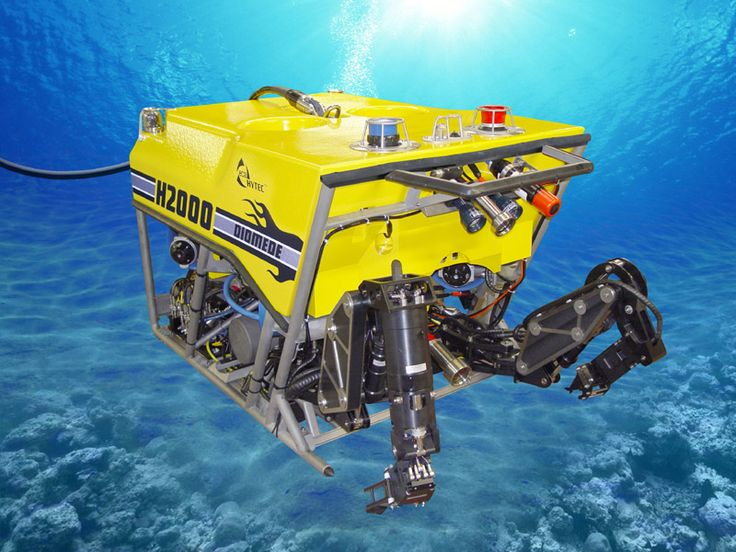
\includegraphics{rov}}}{VPlayer.swf}
        \end{columns}
%*----------- notes
    \note[item]{Notes can help you to remember important information. Turn on the notes option.}
\end{frame}
%-
%*----------- SLIDE -------------------------------------------------------------
\begin{frame}[t]{Questões de Pesquisa}
    \transboxout[duration=0.5]
    \begin{columns}
        \column{.05\textwidth}
        \column{.45\textwidth}
            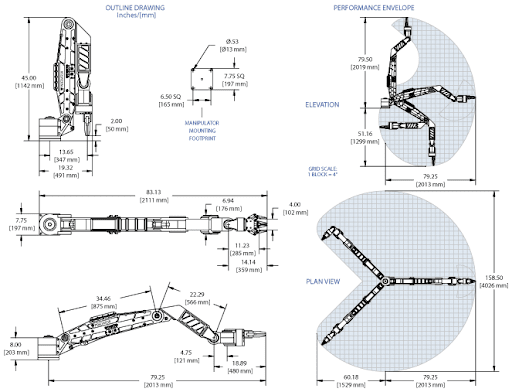
\includegraphics[width=1.1\textwidth]{blueprint-arm}
        \column{.4\textwidth}
            \begin{enumerate}
                \item De que forma as perturbações podem ser compensadas num manipulador submarino?
                \item Qual o modelo para uma melhor eficiência de trajetórias?
                \item Quais variáveis são preponderantes para um controle de trajetórias?
                \item Como estas variáveis podem interferir num novo modelo?
            \end{enumerate}
    \end{columns}
%*----------- notes
    \note[item]{Notes can help you to remember important information. Turn on the notes option.}
\end{frame}
%-
%*----------- SLIDE -------------------------------------------------------------
\begin{frame}[c]{Objetivo geral}
    %\transboxin[duration=1,direction=30]
    %\setbeamercolor{background canvas}{bg=yellow}
    \Wider{%
    \begin{shaded}
    \begin{center}
        \resizebox{!}{0.5cm}{%
            Propor um modelo dinâmico para
        }%
        \\
        \vspace*{0.5cm}
        \resizebox{!}{0.7cm}{%
            planejamento de trajetórias.
        }%
    \end{center}
    \end{shaded}
    }%

%*----------- notes
    \note[item]{Notes can help you to remember important information. Turn on the notes option.}
\end{frame}
%-
\begin{frame}[c]{Objetivos específicos}
    %\transboxin[duration=1,direction=30]
    \centering
    \begin{enumerate}
        \item Realizar \textbf{comparação} entre modelos existentes de planejamento de trajetórias.
        \item Implementar \textbf{odometria visual} num manipulador.
        \item \textbf{Integrar} a odometrial visual com o modelo de planejamento de trajetórias.
        \item \textbf{Simular o modelo} no sistema proposto do manipulador.
    \end{enumerate}
%*----------- notes
    \note[item]{Notes can help you to remember important information. Turn on the notes option.}
\end{frame}
%-
\begin{frame}[c]{Categorias Teóricas}
    %\transboxin[duration=1,direction=30]
    \centering
    \begin{columns}
        \column{.02\textwidth}
        \column{.48\textwidth}
        \begin{itemize}
            \item Planejamento de trajetórias.
            \item Odometria visual.
            \item Manipuladores subaquáticos.
            \item Manipuladores autônomos.
            \item Manipuladores subaquáticos autônomos.
            \item Operação submarina autônoma.
        \end{itemize}
        \column{.25\textwidth}
            \centering
            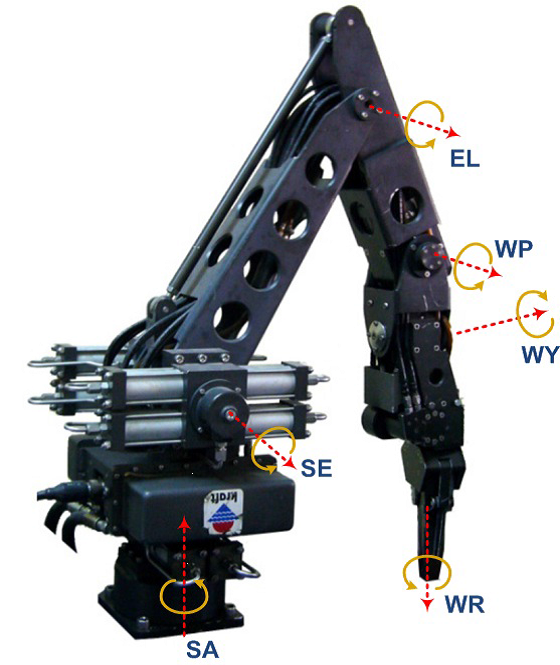
\includegraphics[width=1\textwidth]{kraft}\\
            
\includegraphics[width=.6\textwidth]{apriltag}
        \column{.25\textwidth}
            \centering
            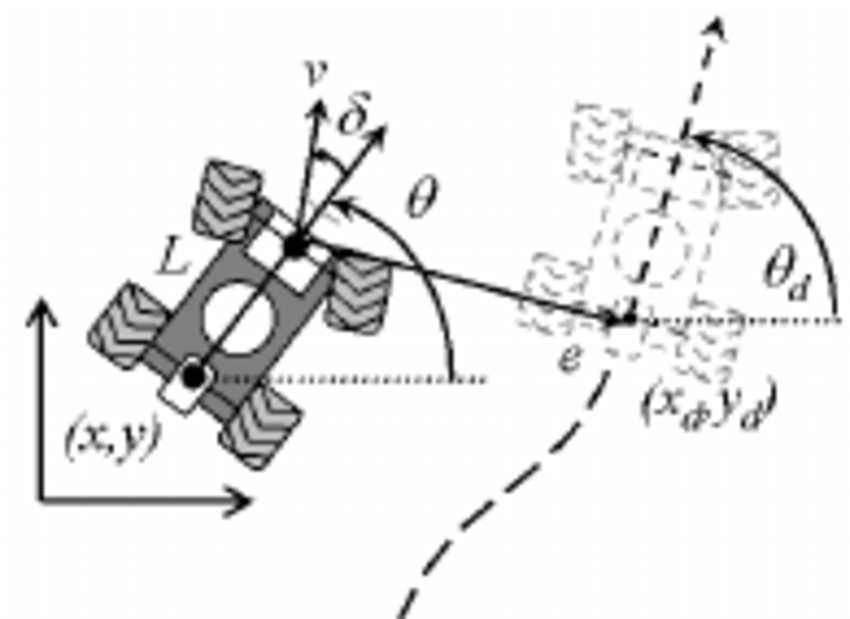
\includegraphics[width=1\textwidth]{visualodom}\\
            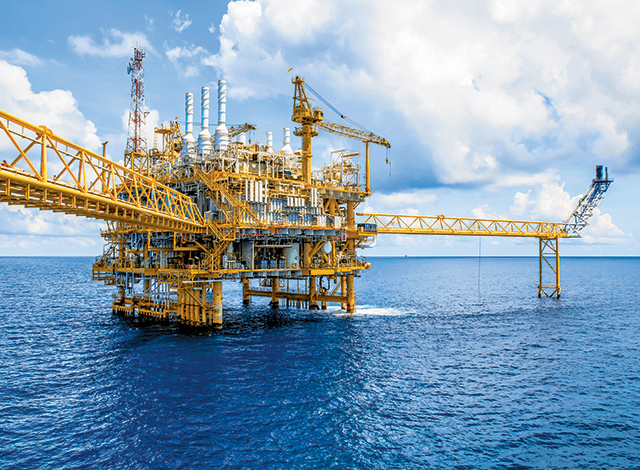
\includegraphics[width=1\textwidth]{opsub}

        % \begin{figure}[ht] \label{ fig7} 
        %     \begin{minipage}[b]{0.5\linewidth}
        %       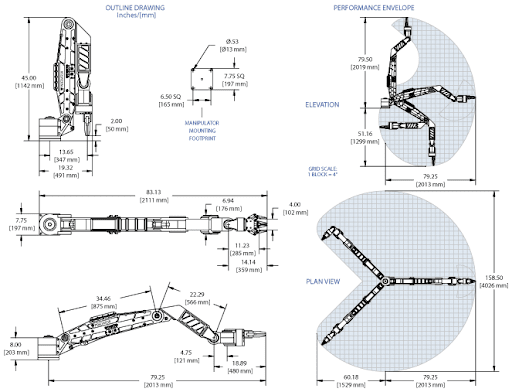
\includegraphics[width=.5\linewidth]{blueprint-arm} 
        %       \caption{Initial condition} 
        %     \end{minipage} 
        %     \begin{minipage}[b]{0.5\linewidth}
        %       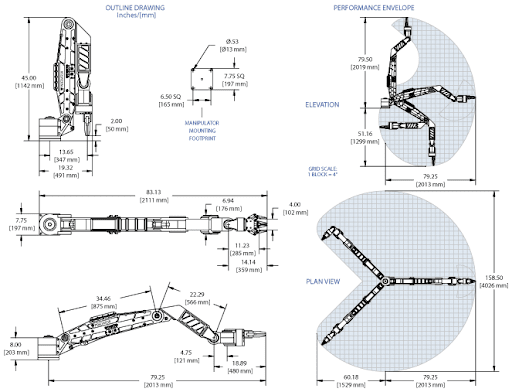
\includegraphics[width=.5\linewidth]{blueprint-arm} 
        %       \caption{Rupture} 
        %     \end{minipage} 
        %     \begin{minipage}[b]{0.5\linewidth}
        %       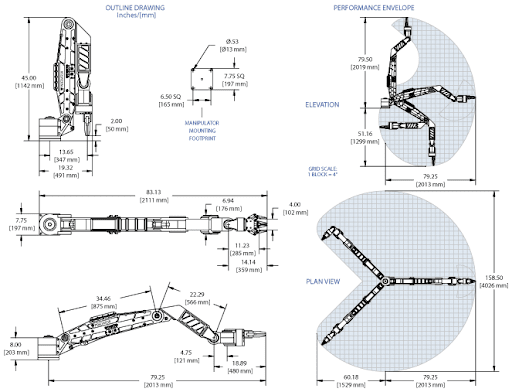
\includegraphics[width=.5\linewidth]{blueprint-arm} 
        %       \caption{DFT, Initial condition} 
        %     \end{minipage}
        %     \hfill
        %     \begin{minipage}[b]{0.5\linewidth}
        %       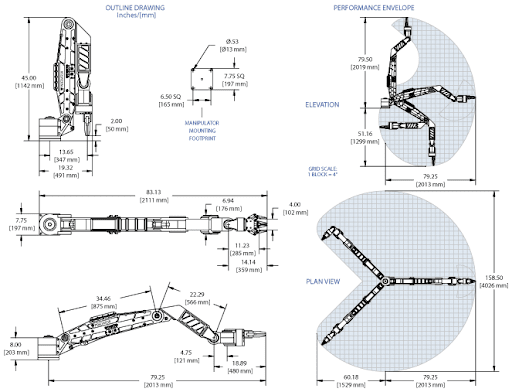
\includegraphics[width=.5\linewidth]{blueprint-arm} 
        %       \caption{DFT, rupture} 
        %     \end{minipage} 
        %   \end{figure}
    \end{columns}
    % \begin{itemize}
    %     \item Planejamento de trajetórias.
    %     \item Odometria visual.
    %     \item Manipuladores subaquáticos.
    %     \item Manipuladores autônomos.
    %     \item Manipuladores subaquáticos autônomos.
    %     \item Operação submarina autônoma.
    % \end{itemize}
    % \begin{block}
    %     {MANIPULADOR}{manipulador}
    % \end{block}

%*----------- notes
    \note[item]{Notes can help you to remember important information. Turn on the notes option.}
\end{frame}
%-
\begin{frame}[c]{Metodologia}
    %\transboxin[duration=1,direction=30]
    \centering
    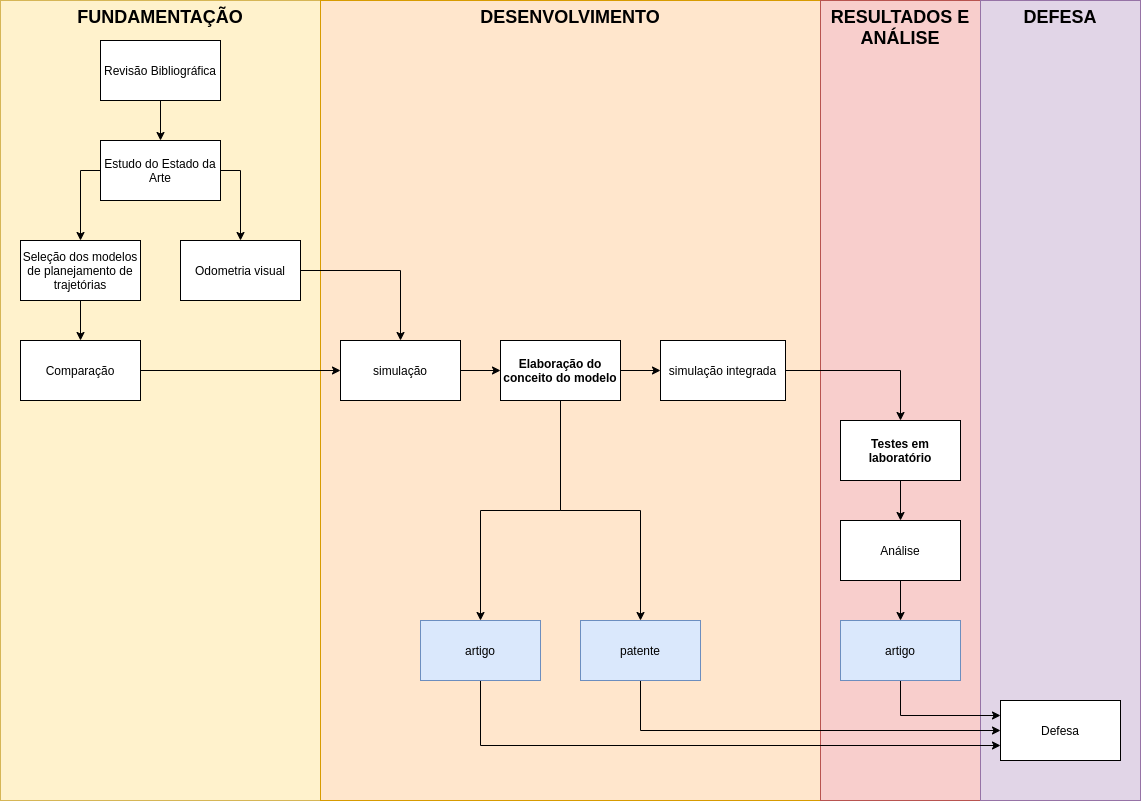
\includegraphics[width=0.7\textwidth]{metodologia11}
%*----------- notes
    \note[item]{Notes can help you to remember important information. Turn on the notes option.}
\end{frame}
%-
\begin{frame}[c]{Cronograma}
    %\transboxin[duration=1,direction=30]
    \centering
    \begin{columns}
        \column{.05\textwidth}
        \column{.95\textwidth}
        % Please add the following required packages to your document preamble:
% \usepackage[table,xcdraw]{xcolor}
% If you use beamer only pass "xcolor=table" option, i.e. \documentclass[xcolor=table]{beamer}
\begin{table}[]
    \begin{tabular}{llllllllllllll|llllllllllll|llllllllllll}
    \cline{3-38}
     & \multicolumn{1}{l|}{} & \multicolumn{12}{c|}{2020} & \multicolumn{12}{c|}{2021} & \multicolumn{12}{c|}{2022} \\ \cline{3-38} 
     & \multicolumn{1}{l|}{} & \multicolumn{1}{c}{J} & \multicolumn{1}{c}{F} & \multicolumn{1}{c}{M} & \multicolumn{1}{c}{A} & \multicolumn{1}{c}{M} & \multicolumn{1}{c}{J} & \multicolumn{1}{c}{J} & \multicolumn{1}{c}{A} & \multicolumn{1}{c}{S} & \multicolumn{1}{c}{O} & \multicolumn{1}{c}{N} & \multicolumn{1}{c|}{D} & \multicolumn{1}{c}{J} & \multicolumn{1}{c}{F} & \multicolumn{1}{c}{M} & \multicolumn{1}{c}{A} & \multicolumn{1}{c}{M} & \multicolumn{1}{c}{J} & \multicolumn{1}{c}{J} & \multicolumn{1}{c}{A} & \multicolumn{1}{c}{S} & \multicolumn{1}{c}{O} & \multicolumn{1}{c}{N} & \multicolumn{1}{c|}{D} & \multicolumn{1}{c}{J} & \multicolumn{1}{c}{F} & \multicolumn{1}{c}{M} & A & M & J & J & A & S & O & N & D \\ \hline
     & \textbf{Disciplinas - cumprimento de créditos} & \textbf{\textgreater{}} & \textbf{\textgreater{}} & \textbf{\textgreater{}} & \textbf{\textgreater{}} & \textbf{\textgreater{}} & \textbf{\textgreater{}} & \textbf{\textgreater{}} & \textbf{\textgreater{}} & \textbf{\textgreater{}} & \textbf{\textgreater{}} & \textbf{\textgreater{}} & \textbf{\textgreater{}} & \textbf{\textgreater{}} & \textbf{\textgreater{}} & \textbf{\textgreater{}} & \textbf{\textgreater{}} & \textbf{\textgreater{}} &  &  &  &  &  &  &  &  &  &  &  &  &  &  &  &  &  &  &  \\ \hline
     & \textbf{Fundamentação} &  &  &  &  &  &  &  &  &  &  &  & \textbf{\textgreater{}} & \textbf{\textgreater{}} & \textbf{\textgreater{}} & \textbf{\textgreater{}} & \textbf{\textgreater{}} & \textbf{\textgreater{}} & \textbf{\textgreater{}} &  &  &  &  &  &  &  &  &  &  &  &  &  &  &  &  &  &  \\ \hline
    1 & Fazer revisão bibliográfica &  &  &  &  &  &  &  &  &  &  &  & \textgreater{} & \textgreater{} &  &  &  &  &  &  &  &  &  &  &  &  &  &  &  &  &  &  &  &  &  &  &  \\
    2 & Elaborar estudo do estado da arte &  &  &  &  &  &  &  &  &  &  &  &  &  & \textgreater{} & \textgreater{} &  &  &  &  &  &  &  &  &  &  &  &  &  &  &  &  &  &  &  &  &  \\
    3 & Comparar modelos pesquisados &  &  &  &  &  &  &  &  &  &  &  &  &  &  & \textgreater{} &  &  &  &  &  &  &  &  &  &  &  &  &  &  &  &  &  &  &  &  &  \\
    4 & Estudar odometria visual &  &  &  &  &  &  &  &  &  &  &  &  &  &  & \textgreater{} & \textgreater{} &  &  &  &  &  &  &  &  &  &  &  &  &  &  &  &  &  &  &  &  \\
    5 & {\color[HTML]{3166FF} \textit{Escrever parte.1 da tese (introdução, fundamentação e metodologia)}} &  &  &  &  &  &  &  &  &  &  &  &  &  & \textgreater{} & \textgreater{} & \textgreater{} & \textgreater{} & \textgreater{} &  &  &  &  &  &  &  &  &  &  &  &  &  &  &  &  &  &  \\
    6 & {\color[HTML]{9A0000} Realizar qualificação} &  &  &  &  &  &  &  &  &  &  &  &  &  &  &  &  &  & \textgreater{} &  &  &  &  &  &  &  &  &  &  &  &  &  &  &  &  &  &  \\ \hline
     & \textbf{Desenvolvimento} &  &  &  &  &  &  &  &  &  &  &  &  &  &  &  &  &  & \textbf{\textgreater{}} & \textbf{\textgreater{}} & \textbf{\textgreater{}} & \textbf{\textgreater{}} & \textbf{\textgreater{}} & \textbf{\textgreater{}} & \textbf{\textgreater{}} &  &  &  &  &  &  &  &  &  &  &  &  \\ \hline
    1 & Realizar simulação dos modelos e odometria &  &  &  &  &  &  &  &  &  &  &  &  &  &  &  &  &  & \textgreater{} & \textgreater{} & \textgreater{} &  &  &  &  &  &  &  &  &  &  &  &  &  &  &  &  \\
    2 & Elaborar conceito do novo modelo &  &  &  &  &  &  &  &  &  &  &  &  &  &  &  &  &  &  &  & \textgreater{} & \textgreater{} &  &  &  &  &  &  &  &  &  &  &  &  &  &  &  \\
    3 & Realizar simulação integrada &  &  &  &  &  &  &  &  &  &  &  &  &  &  &  &  &  &  &  &  & \textgreater{} & \textgreater{} &  &  &  &  &  &  &  &  &  &  &  &  &  &  \\
    4 & {\color[HTML]{3166FF} \textit{Escrever primeiro artigo}} &  &  &  &  &  &  &  &  &  &  &  &  &  &  &  &  &  &  &  &  &  & \textgreater{} & \textgreater{} & \textgreater{} &  &  &  &  &  &  &  &  &  &  &  &  \\
    5 & {\color[HTML]{3166FF} \textit{Escrever patente}} &  &  &  &  &  &  &  &  &  &  &  &  &  &  &  &  &  &  &  &  &  & \textgreater{} & \textgreater{} & \textgreater{} &  &  &  &  &  &  &  &  &  &  &  &  \\ \hline
     & \textbf{Resultados e análise} &  &  &  &  &  &  &  &  &  &  &  &  &  &  &  &  &  &  &  &  &  &  & \textbf{\textgreater{}} & \textbf{\textgreater{}} & \textbf{\textgreater{}} & \textbf{\textgreater{}} & \textbf{\textgreater{}} & \textbf{\textgreater{}} & \textbf{\textgreater{}} & \textbf{\textgreater{}} &  &  &  &  &  &  \\ \hline
    1 & Realizar testes em laboratório &  &  &  &  &  &  &  &  &  &  &  &  &  &  &  &  &  &  &  &  &  &  & \textgreater{} & \textgreater{} & \textgreater{} & \textgreater{} &  &  &  &  &  &  &  &  &  &  \\
    2 & Analisar os dados obtidos &  &  &  &  &  &  &  &  &  &  &  &  &  &  &  &  &  &  &  &  &  &  &  &  &  & \textgreater{} & \textgreater{} &  &  &  &  &  &  &  &  &  \\
    3 & {\color[HTML]{3166FF} \textit{Escrever segundo artigo}} &  &  &  &  &  &  &  &  &  &  &  &  &  &  &  &  &  &  &  &  &  &  &  &  &  &  &  & \textgreater{} & \textgreater{} & \textgreater{} &  &  &  &  &  &  \\ \hline
     & \textbf{Defesa} &  &  &  &  &  &  &  &  &  &  &  &  &  &  &  &  &  &  &  &  &  &  &  &  &  &  &  &  &  & \textbf{\textgreater{}} & \textbf{\textgreater{}} & \textbf{\textgreater{}} & \textbf{\textgreater{}} & \textbf{\textgreater{}} & \textbf{\textgreater{}} & \textbf{\textgreater{}} \\ \hline
    1 & {\color[HTML]{3166FF} \textit{Escrever parte.2 da tese (Resultados e análise e conclusão)}} &  &  &  &  &  &  &  &  &  &  &  &  &  &  &  &  &  &  &  &  &  &  &  &  &  &  &  &  &  & \textgreater{} & \textgreater{} & \textgreater{} & \textgreater{} & \textgreater{} &  &  \\
    2 & {\color[HTML]{9A0000} Realizar defesa perante a banca} &  &  &  &  &  &  &  &  &  &  &  &  &  &  &  &  &  &  &  &  &  &  &  &  &  &  &  &  &  &  &  &  &  &  & \textgreater{} & \textgreater{}
    \end{tabular}
    \end{table}
    \end{columns}

%*----------- notes
    \note[item]{Notes can help you to remember important information. Turn on the notes option.}
\end{frame}
%-
\begin{frame}[c]{Referências}
    %\transboxin[duration=1,direction=30]
    \centering
    
%*----------- notes
    \note[item]{Notes can help you to remember important information. Turn on the notes option.}
\end{frame}
%-